\documentclass[english,11pt,letterpaper,onecolumn]{scrartcl}
%\usepackage{tocloft}
\usepackage[latin1]{inputenc}
\usepackage{csquotes}
\usepackage{stdclsdv}
\usepackage{comment}
\usepackage{vmargin}
\usepackage{t1enc}
\usepackage{fancyvrb}
\usepackage{url}
\usepackage{calc}
\usepackage{array}
\usepackage{scrlayer-scrpage}
\usepackage{graphicx}
\usepackage{color}
\usepackage{listings}
\usepackage[english]{babel}
\usepackage{supertabular}
\usepackage[pdftex,
colorlinks=true,
linkcolor=blue,
pdfpagelabels,
pdfstartpage=2
]{hyperref}
\pagestyle{scrheadings}
\definecolor{LstColor}{cmyk}{0.1,0.1,0,0.025} 
\usepackage[
backend=biber,
style=numeric,
sorting=ynt,
hyperref=true,
backref=true
]{biblatex}

\addbibresource{../gogins.bib}

\begin{document}
\lstset{language=c++,basicstyle=\ttfamily,commentstyle=\ttfamily,tabsize=4,breaklines,backgroundcolor=\color{LstColor},fontadjust=true,keepspaces=false,fancyvrb=true,showstringspaces=false,moredelim=[is][\textbf]{\\emph\{}{\}}}.
\title{Hearing Audio Quality in Csound}
\date{}
\author{Michael Gogins \\ \texttt{michael.gogins@gmail.com}}
\maketitle
\begin{abstract}
This article describes some \emph{methods} for improving the audio quality of Csound pieces, and also a \emph{methodology} for evaluating audio quality and improving one's hearing by using a software-based ABX comparator.
\end{abstract}

Hearing is like thinking: you think you are thinking, but if you go to school 
and study with a good teacher of thinking, you learn that you only 
\emph{thought} you were thinking. Similarly, the naive ear hears things that 
are not there --- things one hopes to hear, or fears to hear --- and fails to 
hear other things that really are there --- things for which one has not 
consciously and reliably heard a \emph{standard of comparison}.

This article contains two main sections, one much more important than the 
other. 

The first section is a laundry list of techniques that have been found to 
improve the subjective, or artistic, sound quality of ``tape music'' style 
compositions rendered using Csound \cite{csoundhome}. For the most part, 
these techniques have to do with choosing the best opcodes for a particular 
task, avoiding certain signal processing artifacts such as clicking and 
aliasing, and understanding how to balance levels and frequencies for a 
transparent listening experience. 

These techniques cover ground that normally comes under the heading of several 
fields, including software instrument design, musical composition and 
arrangement, and audio mastering.

To illustrate the use of these techniques, I have applied some of them to two 
well-known sample compositions that are distributed with Csound. In the 
\url{Csound/examples} directory, you will find both the original and a 
high-definition rendering of \emph{Trapped in Convert}, and both the original 
and a high-definition rendering of \emph{Xanadu}.

The second section describes a \emph{scientific} approach to discovering the 
\emph{artistic} effect of these and other techniques. One renders the same 
piece twice in almost exactly the same way, differing only by one opcode 
choice, or one level change, or one parameter of some other objective 
technique. One then listens to two renderings of the piece using an ABX 
comparator \cite{winabx}, a small software application. The comparator allows 
you to play a selected segment of sound first from one known source A, then 
from another known source B, and finally from an unknown source X chosen 
completely at random from A or B. One must then guess whether A or B was the 
source of X.

This is an absolutely reliable way of finding out what one actually can and 
cannot hear. Scientifically speaking, it is a double-blind experiment. The 
experimenter (the ABX software) does not know which source was chosen for the 
X segment, and the subject (the listener) also does not know which source was 
chosen. Therefore, there is no opportunity for subjective bias to influence 
the results --- at least, not as long as one does not start throwing out 
results one does not like. (It is surprising how tempting this can become!) 
The binomial theorem gives the likelihood for $N$ trials that one has 
identified X by chance and not skill. It does not take many trials to reduce 
the odds that one has identified X by sheer luck to the vanishing point. 

Even better, because the ABX comparator is so reliable, it can be used to 
learn how to correctly discriminate the smallest perceptible differences. In 
other words, the ABX comparator \emph{teaches one to hear}. That is the real 
reason for using this tool with Csound. And Csound is uniquely well suited to 
it, for in live performance, or even in a recording studio, it is very hard to 
produce two versions of the same piece that differ only in one small parameter. 
But with Csound, all it takes is a text editor.

To illustrate the use of the methodology, I suggest some segments in the two 
renderings of \emph{Trapped in Convert} and \emph{Xanadu} to hear using the 
ABX comparator. I am confident that after getting used to the comparator, 
after only a few trials many listeners will experience a sense of revelation 
--- just as I did.

\section{Audio Quality in Csound}
\label{sec:Audio_Quality_in_Csound}

Currently, studio recording is done to stereo, surround sound (5.1 or 7.1), or 
Ambisonics on computers, or hard disk recorders using 24-bit or floating-point 
samples at a rate of 48,000, 88,200, 96,000 or even 192,000 sample frames per 
second. This is ``high-definition audio.'' Analog tape recorders also are still 
sometimes used, and can also be high-definition, if run at high speed and/or 
with noise reduction.

CD-quality audio is of rather lower definition: stereo sound 
with 16 bit integer samples at 44,100 samples per second. 

At the present time, the only consumer electronics formats that can reproduce 
high-definition audio are, roughly in increasing order of quality:
\begin{enumerate}
 \item AAC (the audio part of MP4s) at high bit rates and depths.
 \item SACD (i.e., DSD).
 \item DVD-Audio or, alternatively, DVD-Video containing high-resolution audio.
 \item High-definition PCM soundfiles, or lossless encodings of them 
such as FLAC, ALE in an Ogg Vorbis container, or ALE in an MP4 container.
\end{enumerate}

Right now, the closest thing to a ``universal'' format for high-definition 
audio is Apple Lossless Encoding (ALE) in an MP4 container. This can hold  
both high-resolution video and lossless high-resolution audio. It will play on 
many devices and computers, but does not appear to be supported on YouTube. 

I hope that will change, because YouTube is becoming the most common way 
for most people to listen to music. For YouTube, first produce a 
high-resolution PCM soundfile, then convert it to an MP4 video with 
high-resolution AAC. This, streamed from YouTube, can provide better than CD 
quality.

High-definition audio, on good speakers or earphones, sounds distinctly airy, 
present, spacious, and undistorted. CD-quality audio, by contrast, can sound 
flat, shrill, harsh, and flat or boxed in. Usually, this is the result of 
cumulative mistakes made in this less forgiving medium -- CDs actually are 
precise enough to reproduce most of what we hear. Therefore, CDs made by 
experts can sound very good indeed, except for their more limited dynamic range 
and slightly less detailed quiet sounds. Normally, it takes educated ears to 
hear these differences.

Vinyl records of high quality are not directly comparable to digital 
recordings. They have their own virtues and flaws. They are more detailed, 
airy, and spacious than CDs, but can have harmonic distortion, rumbling, hiss, 
and crackling.  In general, well-made records, especially if pressed 
on thick vinyl from direct metal masters, are roughly equal to high-definition 
audio in aesthetic quality, even if they are not really as precise. 

All of these remarks set aside questions of ``warmth'' or ``musical quality'' 
in sound. Vinyl records, audio tape, and analog electronics introduce a little 
harmonic distortion, which creates a soft, burnished glow on the sound that 
some people prefer to hear. Such ``warmth'' is not what this article is about. 
If the composer or producer wants this sound, it can can easily be created 
using Csound alone, without any analog gear, simply by convolving the signal 
with an appropriate impulse response.

Csound is eminently capable of high-definition audio. It can render to 
\emph{any} number of channels, at \emph{any} sampling rate, using 
floating-point samples. Csound also contains high-quality software 
implementations of all the effects applied by mastering engineers. Therefore, 
Csound can sound as good or better than the best studio gear. However, this 
does \emph{not} happen by default. It takes a little work, and that is what this 
essay is about.

If you have a professional or semi-professional audio interface on your 
computer, you can play high-definition soundfiles made with Csound, although 
you will not hear their full dynamic range unless you have professional 
monitoring gear.

The constant goal in critical listening is to \emph{hear as accurately as 
possible the signal as it actually exists on the recording}. Similarly, the 
constant goal in audio production is not to make a piece sound good on a 
typical listener's sound system --- it is to \emph{make the piece sound as 
good as possible on the most accurate possible listening system}. If you lose 
sight of these realities for any reason, then whether you know it or not, you 
will become lost in a wilderness of illusions. Experienced mastering engineers 
know that making a piece sound good on the most accurate possible sound system 
will make the piece sound better on most listeners' systems and worse on a 
few, whereas trying to make the piece sound good on one sort of inferior sound 
system will indeed make the piece sound much better on that one type of 
system, but only at the cost of making it sound much worse on almost all other 
systems.

I strongly recommend that you listen to all soundfiles from this article 
through real studio monitor speakers, with the flattest possible frequency 
response, in an acoustically deadened room, at a volume that is about as loud 
as you can listen to indefinitely (around 80 dBSP). If you don't have such a 
listening environment, then use real studio monitor headphones plugged into a 
high-definition interface, but be careful not to listen at too high a level.

Specific technical advice in decreasing order of importance (all this assumes 
you don't care how long it takes to render a piece, only if it sounds good):

\begin{enumerate}
	\item Some of the sounds made by Csound have no counterpart in other kinds 
of music. They may contain excessive high frequencies, aliasing distortion, or 
other kinds of noise. On the other hand, the sounds can be of extreme clarity 
and precision --- \emph{hyper-real}. You need to be constantly aware of what 
your sounds \emph{actually sound like}.
	
	\item Always render to floating-point soundfiles at 96,000 sample frames 
per second. You can translate them to 24 bits or to CD quality later if you 
want, but having the extra precision and dynamic range is vital. 

	\item If you use sampled sounds, use the best samples you can possibly 
find. Pay if you must!
	
	\item Also if you use sampled sounds, beware of their own ambience 
clashing with any reverberation or other ambience you set up using Csound. 
Samples may also have unwanted noise --- it may be possible to de-noise them 
(Csound has facilities for doing this too).

	\item Use a ``de-clicking'' envelope to wrap all your instrument final 
output signals.

	\item Watch out for aliasing, which can make sounds buzzy or harsh, in 
frequency modulation and wavetable oscillators. Aliasing happens when the 
signal contains frequencies above half the sampling rate (the Nyquist 
frequency), so that under digital sampling they reflect or fold back under the 
Nyquist frequency. For so-called ``analog'' sounds with simple waveforms such 
as square or sawtooth waves, use non-aliasing opcodes such as \texttt{vco} or 
\texttt{vco2}. You do not need to worry about aliasing with plain sine or 
cosine waves.

    \item Use a-rate variables for envelopes and, in general, wherever opcodes 
permit. This enables decent results with \texttt{ksmps = 100} or so.

\item For final renderings, always render with \texttt{ksmps = 1}. If you 
use a-rate envelopes this may not be not necessary. With \texttt{ksmps > 1}, render 
with the \lstinline{--sample-accurate} option.
	
	\item In general, if an opcode has both an interpolating form and a 
non-interpolating form, use the interpolating form, e.g.\ use \texttt{tablei} 
instead of \texttt{table}.
	
	\item Use only the most precise interpolating oscillators, e.g.\ use
\texttt{poscil3} instead of \texttt{oscil}.

	\item For all wavetable oscillators, the larger the wavetable, the less 
noisy the signal. For each doubling of wavetable size, 
the noise goes down by about 6 dB. For 65536, the noise floor is about -96 dB.

	\item Be vigilant for artifacts and noise introduced by various digital 
signal processing algorithms, especially echoes in reverberation. Don't 
over-use effects --- this is a very common error that you can fix by listening 
to good examples of studio and live recording.

	\item Try rendering with dither (\texttt{-Z} option).

	\item Experiment with some modest compression, e.g.\ by using the 
\texttt{compress} or \texttt{dam} opcodes.

  	\item Use the 64-bit sample version of Csound (this is now standard).
  	
  	\item For final (also known as ``reference'') monitoring, if you must 
  	listen in a smallish room with near-field monitors as most of us do, start all 
  	listening at a C-weighted dBSPL of between 75 and 85, closer to 75, and your digital 
  	signal should be about -20 dBSPL; this level should basically go all the way 
  	down the signal chain. Here is more on that: \url{https://www.soundonsound.com/techniques/establishing-project-studio-reference-monitoring-levels}.
\end{enumerate}

The above are \emph{technical} considerations. \emph{Artistic} considerations 
are more subjective, but the following rules of thumb are generally followed 
in music production:

\begin{enumerate}

	\item For art music that is not acousmatic, the use of signal processing 
and effects should be minimized. In general, the listener should not be aware 
that such effects have been used. If they are audible to the listener, they 
should normally be perceived as being an integral part of a particular voice.

    \item For acousmatic music that uses processed sound, listen very 
critically; avoid using the same processing on all sounds, and avoid the 
almost inevitable builidup of convolution smear.
	
	\item If more than one voice is sounding at the same time, the composer 
usually intends either to fuse the sounds, or to separate the sounds. To fuse 
the sounds, their spectra should overlap, their spatial locations should 
overlap, and their pitches should either be a unison, or in an octave 
relationship. Their envelopes may or may be the same shape, but the attack 
portions should not be too different. To separate sounds, any one or more of 
the above considerations should be negated: their spectra should not overlap; 
and/or their spatial locations should be different; and/or their pitch-classes 
should be different; and/or their envelopes should not be the same shape.
	
	\item Usually, solo voices and bass lines should be acoustically separated 
from the rest of the music.
	
	\item Computer music and electroacoustic music tends to be shrill in 
comparison with historical traditions for art music. Many such pieces can be 
improved by rolling off the treble equalization or, better yet, changing the 
design of the instruments themselves.
	
	\item Computer music and electroacoustic music tends to be bass-shy in 
comparison with other genres of music. Many such pieces can be improved with a 
little ``big bottom.''
	
	\item Computer music and electroacoustic music tends to be loud in 
comparison with other genres of music, excepting the louder forms of rock and 
dance music. Some such pieces would benefit from a quieter average level 
combined with a larger dynamic range.
	
	\item Both computer music and electroacoustic music use a great deal of 
signal processing, which often causes pieces to acquire a particular artifact 
technically known as ``convolution smear.'' It can sound like smearing, 
ringing, or a sheen overlaying the sound. This sound may or may not be 
artistically desirable, but the composer needs to know when it is there so 
that he or she can decide whether or not to use it.
	
	\item Computer music, as opposed to purely electronic music, uses digital 
signal processing which, in turn, frequently causes aliasing distortion. It 
can manifest itself as false tones, false harmonics, or graininess or 
grittiness in sounds. Again, the effect may or may not be desirable, but the 
composer needs to know when it is there.

	\item Computer music, electroacoustic music, and studio recordings in 
general tend to combine sounds into an artificial sound stage. Our sensation 
of the location of sounds is complex, rather accurate, and depends on several 
cues including the relative \emph{loudnesses} of a sound with respect to 
direction, the relative \emph{phases} of the sound with respect to different 
directions, the type of echoes or reverberation associated with the sound, and 
even the frequency equalization of the sound (high frequencies are attenuated 
by distance), not to mention Doppler effects as sound sources move through 
space. Most recorded music features a collapsed, artificial, static sound stage. 
In computer music and electroacoustic music, especially when using sampled 
sound, it is common to use only relative loudness as a spatial cue, and to 
attempt to place sounds with quite different reverberant qualities onto the 
same sound stage. Again, this may or may not be desirable, but the composer 
needs to hear what the sound stage actually is, and to be able to identify its 
causes....
	
\end{enumerate}

\section{Using the ABX Comparator}
\label{sec:Using_the_ABX_Comparator}

There used to be a useful free ABX comparator that could be downloaded from  
\url{http://www.kikeg.arrakis.es/winabx}. This no longer appears to be 
available. I have therefore created a new version of this application,
which can be downloaded from \url{https://github.com/gogins/python-abx}.

In the \url{Csound/examples} directory, you 
will find both the original and high-definition versions of \emph{Trapped in 
Convert} and  \emph{Xanadu}:

\begin{lstlisting}
trapped.csd
trapped-high-resolution.csd
xanadu.csd
xanadu-high-resolution.csd
\end{lstlisting}

\noindent If you do not find these files in your installation of Csound, you 
can download them directly from the Csound GitHub repository at 
\url{https://github.com/csound/csound/tree/develop/examples}.

To see what changes I have made to improve sound quality in these pieces, you 
can run a program such as WinMerge \cite{winmerge} to highlight the 
differences between versions, as shown in Figure \ref{fig:winmerge}.

\begin{figure}[!htp]
	\centering
		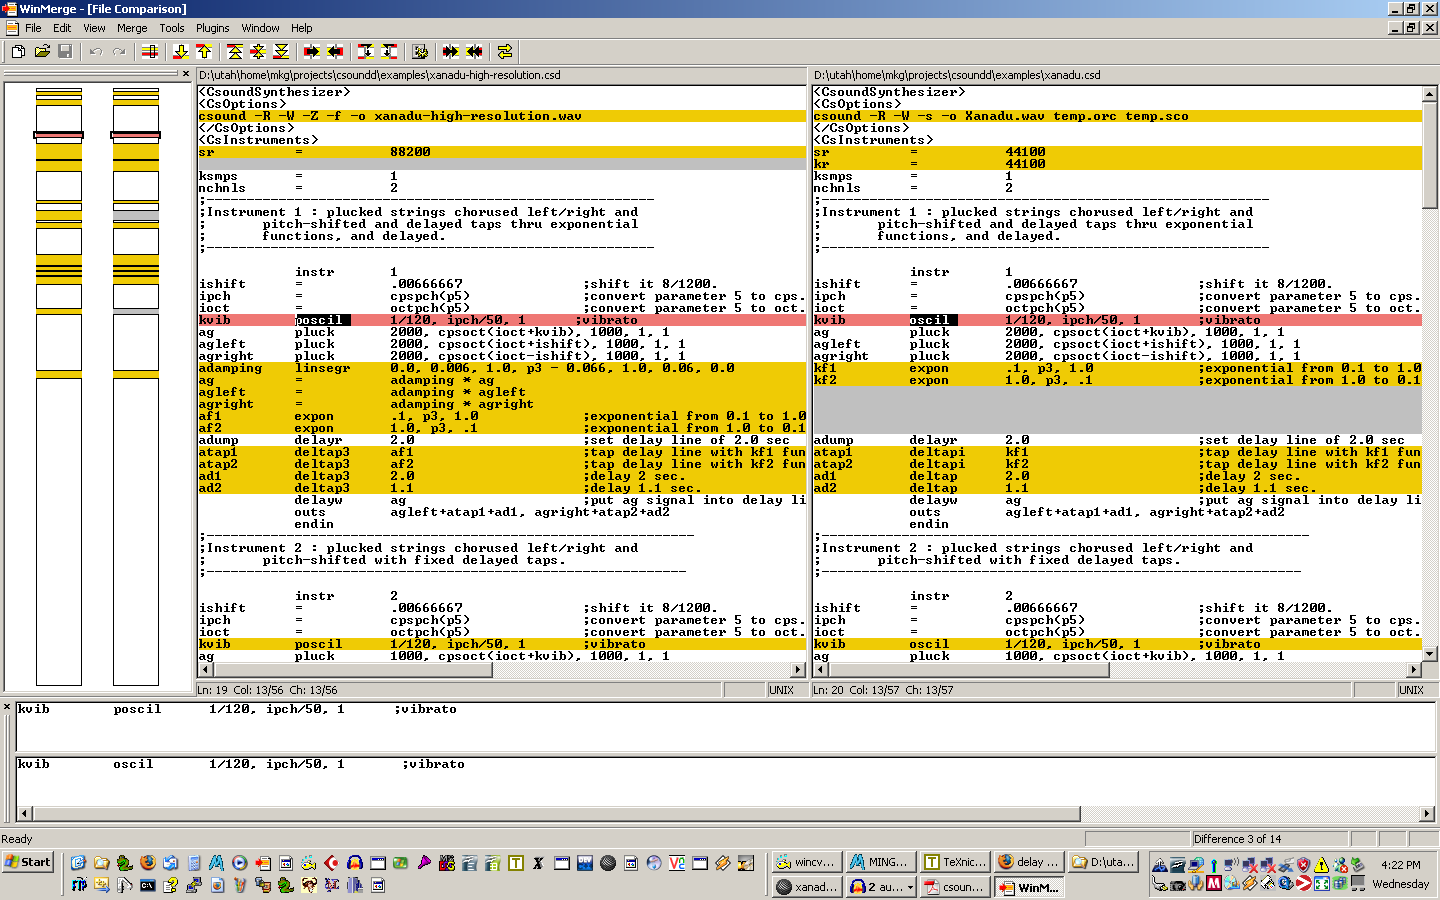
\includegraphics[width=1.0\textwidth]{winmerge.png}
	\caption{\textbf{Comparing Versions of \emph{Xanadu}}}
	\label{fig:winmerge}
\end{figure}

Open a Windows console, navigate to your \url{Csound/examples} directory, and 
render each of the two pieces in both the normal version and the 
high-definition version, using the following commands:

\begin{lstlisting}
csound -R -W -s -o trapped.wav trapped.csd 
csound trapped-high-resolution.csd
csound -R -W -s -o xanadu.wav xanadu.csd
csound xanadu-high-resolution.csd
\end{lstlisting}

Use a soundfile editor such as Audacity \cite{audacity} to determine if the 
soundfile amplitudes are the same in both renderings -- which means within 
0.25 dB of each other. If, but \emph{only} if, the amplitudes of the renderings 
are different, then use the editor to remove any DC bias, and normalize the 
level in each of these soundfiles to -3 dBFS, to ensure that each source has 
the same subjective loudness, as shown in Figure \ref{fig:normalize}. 

Equal amplitudes are \emph{essential} whenever you do an ABX comparison, 
because:

\begin{figure}[!htp]
	\centering
		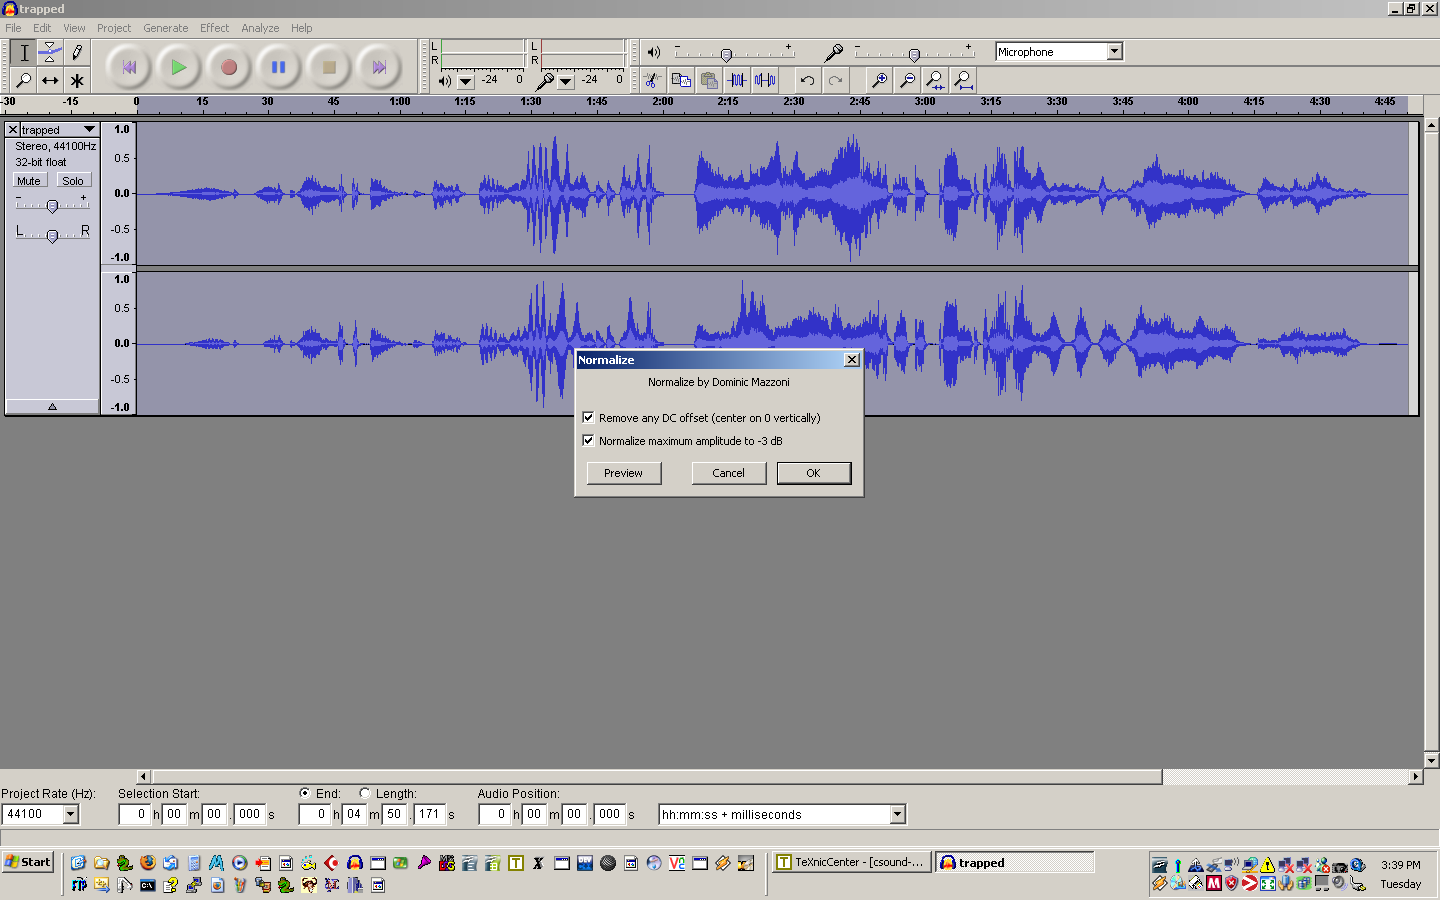
\includegraphics[width=1.0\textwidth]{normalize.png}
	\caption{\textbf{Normalizing \emph{Trapped in Convert}}}
	\label{fig:normalize}
\end{figure}

\begin{itemize}
	\item People are \emph{quite} sensitive to loudness.
	\item Given two sounds A and B, if A is louder, people will tend to prefer 
it, even if at the same loudness they might prefer B.
	\item Different synthesis and signal processing techniques, e.g.\ 
compression, can modify signal amplitudes.
\end{itemize}

When all of your pieces are rendered and, if necessary, normalized, run the 
ABX comparator and load the two versions of \emph{Trapped in Convert}. Select a 
segment beginning at 8 seconds and ending at 10 seconds. The reason for using 
such a short segment is that human short-term memory for sounds is much more 
accurate than long-term memory, and short-term memory only extends to about 5 
seconds. Make sure that your listening volume is loud, but not uncomfortable. 
If while listening your ears hurt or pop, \emph{immediately} reduce the volume
until they do not.

Listen to A and B several times to see if you think you can hear any 
differences between them. Then, listen to X and decide whether X is A or B. 
You are free to listen to A, B, and X any number of times and in any order. I 
find that the best approach is to listen to A and B repeatedly until some 
feature that is different begins to emerge from the listening process. I can 
then listen to X and see if it does or does not have this discriminating 
feature.

When you have made up your mind, click on the \textbf{X is A} button or the 
\textbf{X is B} button to indicate your choice, then click on the \textbf{Next 
trial} button. Keep repeating these trials. If after 10 or 20 trials the 
probability that you are guessing goes below 5\% and stays there, then you 
probably actually \emph{can} hear a difference between A and B. But if 
after a large number of trials you can never get the probability you are 
guessing to stay below 10\%, then no matter what you may think, you probably  
\emph{cannot} hear any difference between A and B. Figure \ref{fig:winabx} 
shows WinABX in action.

\begin{figure}[!htp]
	\centering
		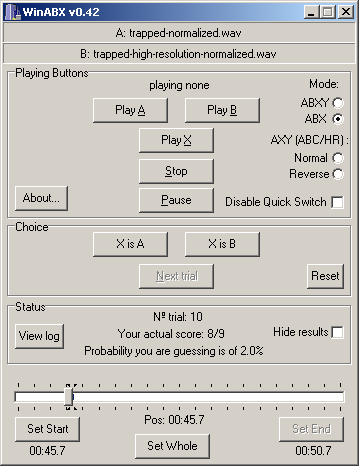
\includegraphics[width=0.5\textwidth]{winabx.png}
	\caption{\textbf{Using WinABX}}
	\label{fig:winabx}
\end{figure}

This is painstaking work, but it is the \emph{only} way to make sure you 
really \emph{are} hearing what you \emph{think} you are hearing.

As time goes on, you should find that your hearing of this piece becomes quite 
a bit more perceptive. More importantly, you should be able to form a reliable 
judgment of which rendering is better according to your own musical taste. 
This may or may not be the high-definition version! \emph{The vital thing is 
to improve the accuracy of your hearing with respect to your own musical 
judgment.} 

You also should find that you can more quickly decide whether or not you 
really can hear a difference between the sources --- which means that you 
really are improving your musical hearing.

I will not, in this article, explain what I think the differences are between 
the regular rendering and the high-definition rendering of \emph{Trapped in 
Convert}. But, here are some other segments to try. 

Warning: not all segments have differences that I could hear!

\begin{enumerate}
	\item 0:46 to 0:51
	\item 1:08 to 1:15
	\item 1:18 to 1:21
	\item 1:53 to 1:56
	\item 2:20 to 2:25
	\item 3:44 to 3:48
	\item 4:28 to 4:32
\end{enumerate}

\noindent When you have listened to a number of segments, you may wish to try 
listening to each version all the way through, in order to see if you can 
still hear the differences that you had learned to identify.

For \emph{Xanadu}, compare the following segments.

Warning: in every case, I \emph{can} reliably hear a difference between the 
renderings!

\begin{enumerate}
	\item 0:00 to 0:02
	\item 0:05 to 0:07
	\item 0:14 to 0:17
	\item 0:23 to 0:24
	\item 0:35 to 0:38
	\item 0:43 to 0:48
	\item 0:51 to 0:55
\end{enumerate}

Of course, your experience with ABX so far concerns two sources that differ by 
many changes in the Csound code. 

If you \emph{really} want to understand what is doing on, make copies of 
\url{trapped.csd} and \url{xanadu.csd}, use a diff tool to add one modification 
at a time to your copies from \url{trapped-high-resolution.csd} and 
\url{xanadu-high-resolution.csd} files, and do the ABX comparison all over for 
each modification.

Another source of deeper insight might be to visit Dominique Bassal's web site 
on mastering \cite{bassal_mastering}, download some of his 
pre-mastered/post-mastered example soundfiles, and do ABX comparisons on them. 
Bassal is an acknowledged expert in mastering computer music, and his on-line 
article \emph{The Practice of Mastering in Electroacoustics} 
\cite{bassal_mastering_pdf} provides a much more experienced and in-depth 
review of some of the issues (i.e., those not specific to Csound) that I have 
tried to cover here.

\section{Conclusion}

Well, I hope this article has been useful to you!

I believe that learning these methods, and above all the ABX methodology, has 
made an enormous difference to my own ability to hear my own music more 
objectively. 

I also have a renewed appreciation of what I am now better equipped to realize 
are astonishing feats of perception and signal processing on the part of the 
best computer musicians, recording engineers, and mastering engineers. 

And I believe my own ability to work at that level has improved, at least a 
little bit, as a result of the ABX comparator.

\printbibliography

\end{document} 

